\documentclass{llncs}

\usepackage{graphicx}

\newcommand{\ignore}[1]{}

\begin{document}

\title{Designing Oligonucleotide Microarrays (provisional title)}
%
% abbreviated title (for running head) also used for the TOC unless \toctitle is used
\titlerunning{Designing Oligonucleotide Microarrays}
%
\author{Sergio A. de Carvalho Jr.\inst{1,}\inst{2} \and Sven Rahmann\inst{2,}\inst{3}}
%
% abbreviated author list (for running head)
\authorrunning{de Carvalho Jr. and Rahmann}
%
%%%% modified list of authors for the TOC (add the affiliations)
\tocauthor{Sergio A. de Carvalho Jr. (Universit\"{a}t Bielefeld),
Sven Rahmann (Universit\"{a}t Bielefeld)}
%
\institute{Graduiertenkolleg Bioinformatik, Bielefeld University, Germany \\
\email{Sergio.Carvalho@cebitec.uni-bielefeld.de}
\and
International NRW Graduate School in Bioinformatics and Genome Research,
Bielefeld University, Germany
\and
Algorithms and Statistics for Systems Biology group, Genome Informatics,
Technische Fakult\"at, Bielefeld University, D-33594 Bielefeld, Germany \\
\email{Sven.Rahmann@cebitec.uni-bielefeld.de}
}

% typeset the title of the contribution
\maketitle

% The abstract should summarize the contents of the paper
% using at least 70 and at most 150 words. It will be set in 9-point
% font size and be inset 1.0 cm from the right and left margins.
% There will be two blank lines before and after the Abstract.
\begin{abstract}
The production of commercial DNA microarrays is based on a
light-directed chemical synthesis driven by a set of masks or
micromirror arrays. Because of the natural properties of light and the
ever shrinking feature sizes, the arrangement of the probes on the
chip and the order in which their nucleotides are synthesized play an
important role on the quality of the final product. We propose a new
model called \emph{conflict index} for evaluating microarray layouts.
\end{abstract}

% ==============================================================================
\section{Introduction}
% ==============================================================================
\label{sec:intro}

An oligonucleotide microarray is a piece of glass or plastic on which
single-stranded fragments of DNA, called \emph{probes}, are affixed or
synthesized. The Affymetrix GeneChip\raisebox{.6ex}{\scriptsize \textregistered}
arrays, for instance, can contain
more than one million spots (or \emph{features}) as small as 11 $\mu$m,
with each spot accommodating several million copies of a probe. Probes
are typically 25 nucleotides long and are synthesized in parallel, on
the chip, in a series of repetitive steps. Each step appends the same
nucleotide to probes of selected regions of the chip. Selection occurs
by exposure to light with the help of a photolithographic mask that
allows or obstructs the passage of light accordingly \cite{FODOR91}.

Formally, we have a set of probes $\mathcal{P} = \{p_{1}, p_{2}, ... p_{n}\}$
that are produced by a series of masks $\mathcal{M} = (m_{1}, m_{2}, ... m_{\mu})$,
where each mask $m_{k}$ induces the addition of a particular nucleotide
$t_{k} \in \{A, C, G, T\}$ to a subset of~$\mathcal{P}$. The \emph{nucleotide
deposition sequence} $\mathcal{S} = t_{1} t_{2} \ldots t_{\mu}$ corresponding
to the sequence of nucleotides added at each masking step is therefore a
supersequence of all $p_{i} \in \mathcal{P}$ \cite{RAHMANN03}.

In general, a probe can be \emph{embedded} within $\mathcal{S}$ in several
ways. An embedding of $p_{i}$ is a $\mu$-tuple
$\varepsilon_{i} = (e_{i,1}, e_{i,2}, ... e_{i,\mu})$ in which $e_{i,k} = 1$
if probe $p_{i}$ receives nucleotide $t_{k}$ (at step~$k$), or 0 otherwise
(Figure~\ref{fig:masking_process}). In particular, a \emph{left-most embedding}
is an embedding of a probe where each base is synthesized as soon as possible.

\begin{figure}
\centerline{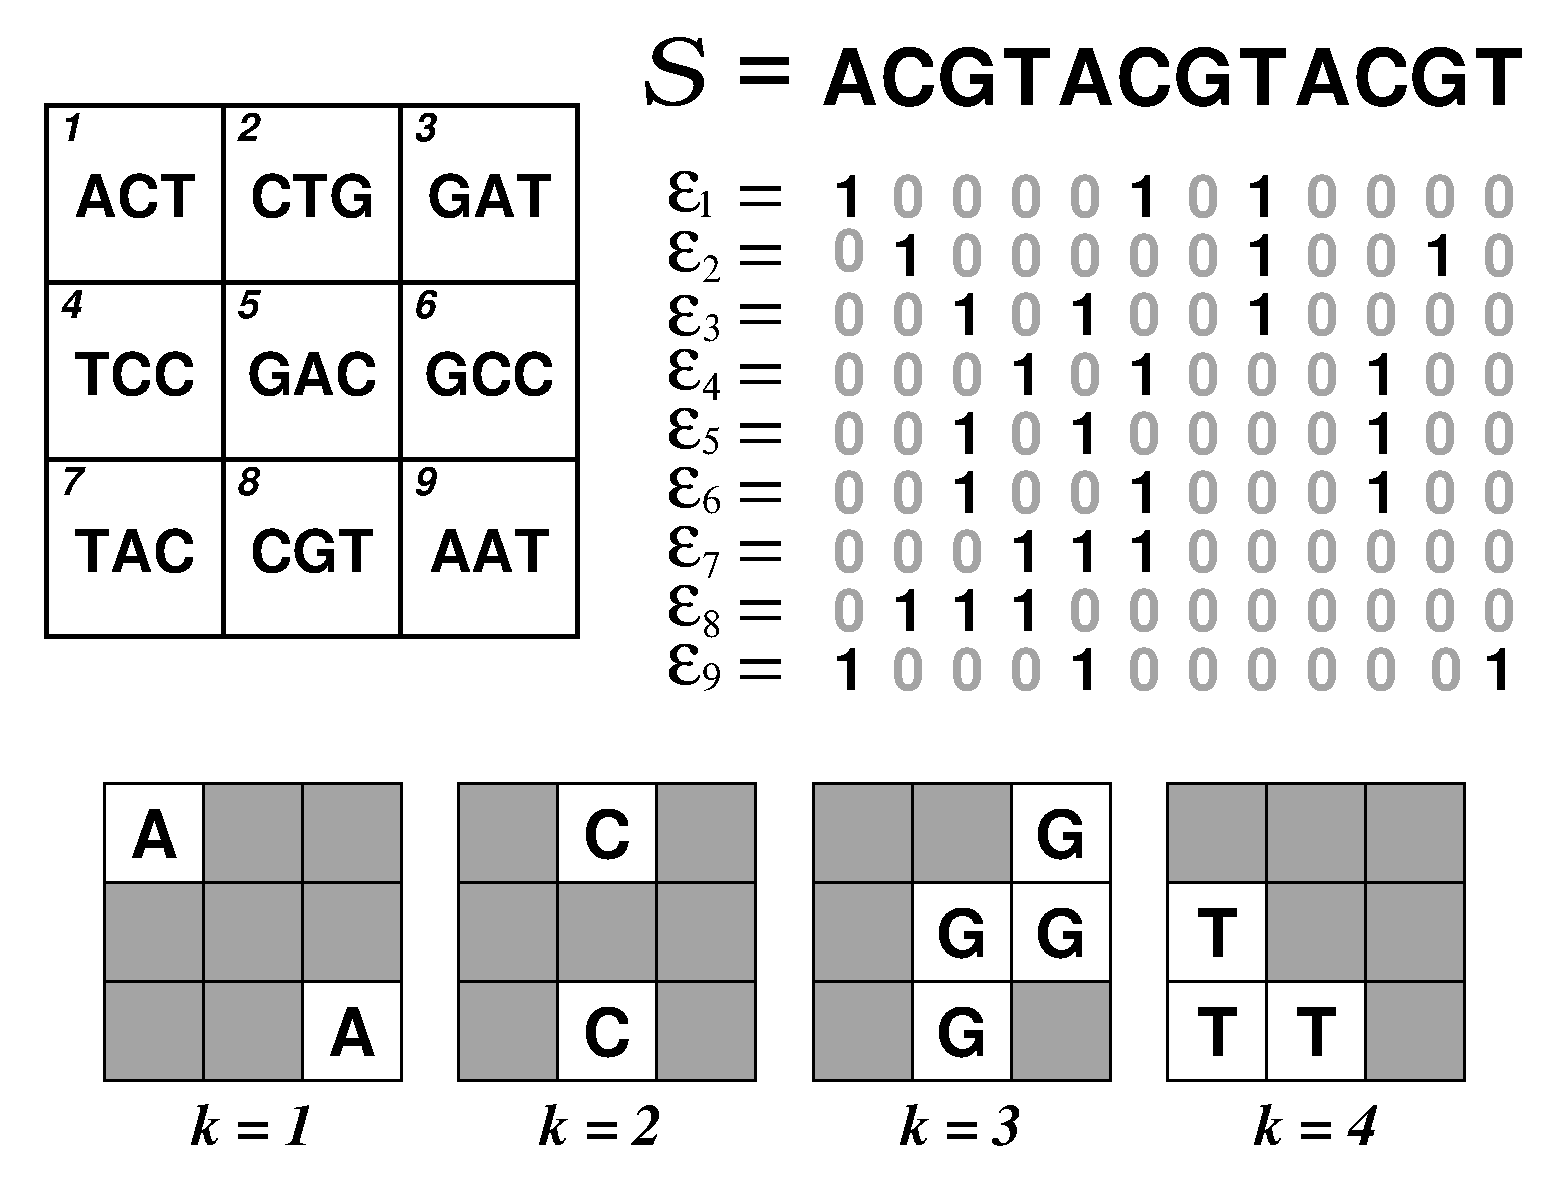
\includegraphics[width=230pt]{chip}}
\caption{Synthesis of a hypothetical 3\,x\,3 chip. On the top left, the chip layout and its 3-base-long probe sequences. On the top right, the deposition sequence and the probe embeddings. On the bottom, the first four resulting photolithographic masks.}
\label{fig:masking_process}
\end{figure}

Deposition sequences are usually cyclical, that is $\mathcal{S}$ is a repeated
permutation of the alphabet. This is mainly because such sequences maximize the
number of possible subsequences \cite{CHASE76}. In this context, we can
distinguish between \emph{synchronous} and \emph{asynchronous} embeddings. In
the first case, each probe has one and only one nucleotide synthesized in every
cycle of the deposition sequence; hence, 100 masking steps are needed to
synchronously synthesize probes of length 25. In the case of asynchronous
embeddings, probes can have any number of nucleotides synthesized in any given
cycle. This allows for shorter deposition sequences. All Affymetrix chips that
we know of can be asynchronously synthesized in 74 masking steps\footnote{We
understand that Affymetrix uses the same truncated repetition of TGCA to
synthesize most (if not all) GeneChip arrays, which suggests that their probe
selection procedure is restricted to sequences that fit into this deposition
sequence.}.

Because of diffraction of light or internal reflection, untargeted spots can
sometimes be accidentally activated in a certain masking step, producing
unpredicted probes that can compromise the results of an experiment. This issue
was described by Fodor~{\it et~al}.~\cite{FODOR91}, who noted that the problem
is more likely to
occur near the borders between masked and unmasked spots. This observation has
given rise to the term \emph{border conflict}.

We are interested in finding an arrangement of the probes on the chip together
with their embeddings in such a way that the chances of unintended
illumination during mask exposure steps is minimized. This problem appears to
be hard (although the authors are not aware of an NP-hardness proof) because
of the exponential number of possible arrangements, and optimal solutions are
unlikely to be found even for very small chips, and even if we consider the probes
as having a single pre-defined embedding.

% TODO should this be mentioned? where?
In a separate work~\cite{CARVALHO06}, we have presented a formulation based on
the quadratic assignment problem (QAP), a classical combinatorial optimization
problem that is known to be NP-hard and NP-hard to approximate. Our formulation
gives further indication that the problem is hard.

If we consider all valid embeddings that a probe can have, the problem is even
harder. Probes
of an Affymetrix chip, for instance, can have up to several million possible
embeddings. For this reason, the problem has been traditionally tackled in two
phases. First, an initial embedding of the probes is fixed and an arrangement of
these embeddings on the chip with minimum border conflicts is sought. This is
usually referred to as the \emph{placement} problem. Second, a \emph{post-placement}
optimization phase re-embeds the probes considering its location on the chip,
in such a way that the conflicts with the neighboring spots are further reduced.

We believe that better solutions can be found if, during the placement, we also
consider the various embeddings that a probe can have. In this paper we present
a new algorithm... % TODO continue...

In the next section, we review the Border Length Minimization Problem
\cite{HANNENHALLI02}, and define an extended model for evaluating microarray
layouts. In Section~\ref{sec:previous_work}, we briefly review existing
placement strategies. % TODO finish this paragraph


% ==============================================================================
\section{Layout Evaluation}
% ==============================================================================
\label{sec:eval}

\subsection{Border Length}

Hannenhalli~{\it et~al}.\ were the first to give a formal definition to the problem
of unintended illumination in the production of microarrays. They formulated the
\emph{Border Length Minimization Problem}\cite{HANNENHALLI02}, which aims at finding
an arrangement of the probes together with their embeddings in such a way the number
of border conflicts during mask exposure steps is minimal.

The \emph{border length}~$\mathcal{B}_k$ of a mask~$m_{k}$ is simply
defined as the number of borders shared by masked and unmasked spots
at masking step~$k$. The total border length of a given arrangement is
the sum of border lengths over all masks. For example, in
Figure~\ref{fig:masking_process}, the four masks shown have
$\mathcal{B}_1 = 4$, $\mathcal{B}_2 = 6$, $\mathcal{B}_3 = 6$ and $\mathcal{B}_4 = 4$.
The total border length of that arrangement is 50.

% ------------------------------------------------------------------------------
\subsection{Conflict Index}

The border length of an individual mask measures the quality of that
mask. We are more interested in estimating the risk of synthesizing a faulty
probe at a given spot. That is, we need a per-spot measure
instead of a per-mask measure. Additionally, Kahng~{\it et~al}.~\cite{KAHNG03A} noted
that the definition of border length does not take into account two
simple yet important practical considerations:
\begin{itemize}
\item[a)] stray light might activate not only adjacent neighbors but
  also probes that lie as far as three cells away from the targeted
  spot;
\item[b)] imperfections produced in the middle of a probe are more
  harmful than in its extremities.
\end{itemize}
This motivates the following definition of the \emph{conflict
  index}~$\mathcal{C}(s)$ of a spot~$s$ whose probe of
length~$\ell_{s}$ is synthesized in $\mu$~masking steps. First we
define a distance-dependent weighting function, $\delta(s,s',k)$, that
accounts for observation a) above:
%%
\begin{equation}
\label{eq:dist_weight}
\delta(s,s',k) :=
        \left\{
                \begin{array}{ll}
                        (d(s,s'))^{-2} & \mbox{if $s'$ is unmasked at step $k$}, \\
                        0 & \mbox{otherwise}, \\
                \end{array}
        \right.
\end{equation}
%%
where $d(s,s')$ is the Euclidian distance between spots~$s$ and~$s'$.
This form of weighting function is the same as suggested in
\cite{KAHNG03A}.  Note that $\delta$ is a ``closeness'' measure
between $s$ and $s'$ only if the spot in the neighboring spot $s'$ is
not masked (and thus creates the potential of illumination at $s$). To
restrict the number of neighbors that need to be considered, we
restrict the support of $\delta(s,s',\cdot)$ to those $s'\neq s$ that
are in a $7\times 7$ grid centered around $s$ (see
Figure~\ref{fig:conflictindex}~top).


We use position-dependent weights to account for observation b):
%%
\begin{equation}\label{eq:pos_mult}
\omega(s,k) :=
        \left\{
                \begin{array}{ll}
                        c \cdot \exp{\left(\theta \cdot \lambda(s,k)\right)} & \mbox{if $s$ is masked at step $k$}, \\
                        0 & \mbox{otherwise}, \\
                \end{array}
        \right.
\end{equation}
%%
where $c>0$ and $\theta>0$ are constants, and
%%
\begin{equation}\label{eq:base_pos}
  \lambda(s,k) := 1 + \min(b_{s,k},\ell_{s} - b_{s,k})
\end{equation}
%%
is the distance of the nucleotide synthesized in step $k$ (if any)
from the start or end of the probe: $b_{s,k}$ denotes the number of
nucleotides synthesized at spot~$s$ up to and including step~$k$ and
$\ell_s$ is the probe length (see Figure~\ref{fig:conflictindex}
bottom). We set the constants $c$ and $\theta$ as follows:
\[ \theta = \frac{5}{\ell_s}; \qquad c = \frac{1}{\exp{\theta}}. \]
It is generally agreed that the chances of a successful hybridization
between probe and target are higher if a mismatched base occurs at the
extremities of the formed duplex instead of at its center. The precise
effects of this position, however, is not yet fully understood and has
been an active topic of research \cite{BINDER05}. The motivation
behind an exponentially increasing weighting function is that the
probability of a successful stable hybridization of a probe with its
target should increase exponentially with the absolute value of its
Gibbs free energy, which increases linearly with the length of the
longest perfect match between probe and target. The parameter $\theta$
controls how steeply the exponential weighting function rises towards
the middle of the probe.

We now define the conflict index of a spot $s$ as
\begin{equation}
\label{eq:conf_idx}
\mathcal{C}(s) := \sum_{k=1}^{\mu} \left( \omega(s,k) \sum_{s'} \delta(s,s',k) \right),
\end{equation}
%%
where $s'$ ranges over all spots that are at most three cells away
from $s$.  $\mathcal{C}(s)$ can be interpreted as the fraction of
faulty probes (because of unwanted illumination) produced at spot $s$.

\begin{figure}
%%
\footnotesize{ \centerline{
\begin{tabular}{c|c|c|c|c|c|c|c|} \cline{2-8}
& \ 0.06 & \ 0.08 & \ 0.10 & \ 0.11 & \ 0.10 & \ 0.08 & \ 0.06 \\ \cline{2-8}
& \ 0.08 & \ 0.13 & \ 0.20 & \ 0.25 & \ 0.20 & \ 0.13 & \ 0.08 \\ \cline{2-8}
& \ 0.10 & \ 0.20 & \ 0.50 & \ 1.00 & \ 0.50 & \ 0.20 & \ 0.10 \\ \cline{2-8}
& \ 0.11 & \ 0.25 & \ 1.00 & \  s   & \ 1.00 & \ 0.25 & \ 0.11 \\ \cline{2-8}
& \ 0.10 & \ 0.20 & \ 0.50 & \ 1.00 & \ 0.50 & \ 0.20 & \ 0.10 \\ \cline{2-8}
& \ 0.08 & \ 0.13 & \ 0.20 & \ 0.25 & \ 0.20 & \ 0.13 & \ 0.08 \\ \cline{2-8}
& \ 0.06 & \ 0.08 & \ 0.10 & \ 0.11 & \ 0.10 & \ 0.08 & \ 0.06 \\ \cline{2-8}
\end{tabular}
}}
%%
\footnotesize{\centerline{
%%
\begin{picture}(415,165)
%% \put(0,123){a)}
%% \put(0,41){b)}
\put(15,0){\makebox(395,165){
%GNUPLOT: LaTeX picture with Postscript
\begin{picture}(0,0)%
\includegraphics{position_weights}%
\end{picture}%
\begingroup
\setlength{\unitlength}{0.0200bp}%
\begin{picture}(9900,5940)(0,0)%
\put(1250,1500){\makebox(0,0)[r]{\strut{} 0}}%
\put(1250,2157){\makebox(0,0)[r]{\strut{} 2}}%
\put(1250,2813){\makebox(0,0)[r]{\strut{} 4}}%
\put(1250,3470){\makebox(0,0)[r]{\strut{} 6}}%
\put(1250,4127){\makebox(0,0)[r]{\strut{} 8}}%
\put(1250,4783){\makebox(0,0)[r]{\strut{} 10}}%
\put(1250,5440){\makebox(0,0)[r]{\strut{} 12}}%
\put(1647,1000){\makebox(0,0){\strut{} 0}}%
\put(3118,1000){\makebox(0,0){\strut{} 5}}%
\put(4589,1000){\makebox(0,0){\strut{} 10}}%
\put(6061,1000){\makebox(0,0){\strut{} 15}}%
\put(7532,1000){\makebox(0,0){\strut{} 20}}%
\put(9003,1000){\makebox(0,0){\strut{} 25}}%
%\put(5325,250){\makebox(0,0){\strut{}$b_{s,k}$}}%
\end{picture}%
\endgroup
\endinput

%%% Local Variables: 
%%% mode: latex
%%% TeX-master: t
%%% End: 

}}
% \includegraphics*[0mm,0mm][128mm,65mm]{division}
\end{picture}\vspace*{-3ex}
%%
}}
%%
\caption{Ranges of values for both $\delta$ and $\omega$ on a typical Affymetrix
chip where probes of length~$\ell = 25$ are synthesized in $\mu = 74$ masking
steps. Top: Distance-dependent weighting function $\delta(s,s',k)$ for a spot~$s$
(shown in the center) and all close neighbors $s'$, assuming that $s'$ is unmasked
at step $k$.  Bottom: Position-dependent weights $\omega(s,k)$ at each value of
$b_{s,k}$, assuming that spot $s$ is masked at step $k$.}
\label{fig:conflictindex}
\end{figure}

Finally, we note the following relation between conflict indices and border
lengths: Define $\delta(s,s',k):=1$ if $s'$ is a direct neighbor of $s$ and is
unmasked in step $k$, and $:=0$ otherwise.  Also define $\omega(s,k):=1$ if
$s$ is masked in step $k$, and $:=0$ otherwise. Then $\sum_s\, \mathcal{C}(s)
= 2 \sum_{k=1}^\mu\, \mathcal{B}_k$, as each border conflict is counted twice:
for $s'$ and $s$.

This shows that total border length and total conflict are correlated. A good
layout is one with low border length as well as low average conflict index,
although it is clearly possible to observe a reduction of the conflict index
at the expense of an increase in border length, and vice-versa.


% ==============================================================================
\section{Previous Work}
% ==============================================================================
\label{sec:previous_work}

We now briefly review existing algorithms, laying the groundwork for our
contribution.

% ------------------------------------------------------------------------------
\subsection{Placement Algorithms}
\label{sec:placement_alg}

\ignore{The first to formally address the border length problem were \cite{FELDMAN93}.
They showed how an optimal placement can be constructed based on a two-dimensional
Gray code. However, their work is restricted to \emph{uniform arrays} (arrays
containing all possible probes of a given length) and synchronous embeddings.}

Hannenhalli~{\it et~al}.\ \cite{HANNENHALLI02} were the first to consider the border
length problem on large
oligonucleotide arrays of arbitrary probes. They reported that the first Affymetrix
chips were designed using a heuristic for the traveling salesman problem (TSP). The
idea consists of building a weighted graph with nodes representing probes and edges
containing the Hamming distance between the probe sequences. A TSP tour is approximated,
resulting in consecutive probes in the tour being likely to be similar. The TSP
tour is then \emph{threaded} on the array in a row-by-row fashion.
Hannenhalli~{\it et~al}.\ suggested a different threading of the TSP tour on the chip,
called \emph{1-threading}, to achieve up to 20\% reduction in border length.

Kahng~{\it et~al}.~\cite{KAHNG02} propose the \emph{Epitaxial} placement algorithm that
places a random probe in the center of the array and continues to
insert probes in spots adjacent to already filled spots, employing a
greedy heuristic to select the next spot to be filled and the probe
that is assigned to it. Priority is given to spots whose
neighbors are already filled, in which case the algorithm places the
probe with minimum sum of Hamming distances to its neighbors. If no
such a spot exists, the algorithm examines all non-filled spots~$s_i$
with $n_i \geq 1$ filled neighbors and finds a non-assigned probe
$p_j$ with minimum sum of Hamming distances to the neighboring probes
$H_{ij}$. For each possible assignment of $p_j$ to $s_i$, it computes
a cost $c(s_i,p_j) := k_{n_i} H_{ij} / n$, where $k_{n_i}$ are scaling
coefficients ($k_1 = 1$, $k_2 = 0.8$, and $k_3 = 0.6$), and makes the
assignment with minimum cost. With this algorithm, they claimed to
achieve up to 10\% reduction in border conflicts over the TSP-based
approach of Hannenhalli~{\it et~al}.\ \cite{HANNENHALLI02}.

\ignore{
The major problem with the Epitaxial and the TSP-based algorithm is that they
have at least quadratic time complexity and thus are not scalable for the
latest million-probe microarrays. According to their experiments, the TSP
approach needed around 32 minutes to produce the layout of a 200\,x\,200
chip, whereas the epitaxial algorithm needed 74 minutes on average. For a
500\,x\,500 chip, the TSP took over 30 hours to complete, whereas the
epitaxial algorithm did not complete ``due to prohibitively large running
time or memory requirements'' \cite{KAHNG02}.
}

\ignore{
This observation has led to the development of two new algorithms by
\cite{KAHNG03A}. The first one, called Sliding-window Matching (SWM), is not
exactly a placement algorithm as it iteratively improves an initial placement
that can be constructed by, for instance, TSP and 1-threading. Improvements
are achieved by selecting an independent set of spots inside the window and
optimally replacing their probes using a minimum-weight perfect matching
algorithm. The term independent refers to probes that can be replaced without
affecting the border length of the other selected probes.
}

Both the TSP and the epitaxial approach do not scale well to large
chips.  Another algorithm described by Kahng~{\it et~al}.~\cite{KAHNG03A} is a variant
of the Epitaxial algorithm, called \emph{Row-epitaxial}, with two main
differences: spots are filled in a pre-defined order, namely
row-by-row, and only probes of a limited list of candidates $Q$ are
considered when filling each spot. Their experimental results showed
that the row-epitaxial is the best large-scale placement algorithm,
achieving up to 9\% reduction in border length when compared to the
TSP-based approach of Hannenhalli~{\it et~al}.\ \cite{HANNENHALLI02}.

% ------------------------------------------------------------------------------
\subsection{Partitioning Algorithms}
\label{sec:partition}

The ever growing number of probes on the latest microarrays and the properties of
the placement problem naturally suggest the use of partitioning strategies to reduce
the running time of the algorithms. The placement problem can be partitioned by
dividing the set of probes into smaller sub-sets, and assigning these sub-sets to
sub-regions of the chip. Each sub-region can then be treated as an independent chip
or recursively partitioned. These smaller sub-problems, when solved, immediately
constitute a final solution. In this way, algorithms with non-linear time or space
complexities can be used to compute the layout of larger chips that otherwise would not
be feasible. A partitioning is clearly a compromise in solution quality. However,
due to the large number of probes, this compromise can be small, specially if the
partitioning is able to place similar probes together.

The only partitioning algorithm available in the literature is the Centroid-based
Quadrisection \cite{KAHNG03B}. It is a recursive procedure that works as follows.
First, it randomly selects a probe $c_1$ from the probe set $\mathcal{P}$. Then,
it examines all other probes of $\mathcal{P}$ and selects $c_2$ with maximum
$h(c_1,c_2)$, where $h(c_1,c_2)$ is the Hamming distance between the embeddings
of $c_1$ and $c_2$. Similarly it finds $c_3$ with maximum $h(c_1,c_3) + h(c_2,c_3)$
and $c_4$ with maximum $h(c_1,c_4) + h(c_2,c_4) + h(c_3,c_4)$. Probes
$c_1$, $c_2$, $c_3$ and $c_4$ are called centroids. All other probes
$p_i \in \mathcal{P}$ are then compared to the centroids and assigned to the sub-set
$\mathcal{P}_j$ associated with $c_j$ with minimum $h(p_i,c_j)$. Each sub-set
$\mathcal{P}_j$ is assigned to a sub-region of the chip. The procedure is repeated
recursively on each sub-region until a given recursion depth is reached.

The result of this algorithm is a partitioning of the chip into several sub-regions
and an assignment of sub-sets of $\mathcal{P}$ to each sub-region. For the actual
placement of the probes in each sub-region, another algorithm is needed. For this
purpose, Kahng~{\it et~al}.~\cite{KAHNG03B} have used the row-epitaxial algorithm
described in the previous sub-section.

% ------------------------------------------------------------------------------
\subsection{Post-placement Optimization}
\label{sec:optimization}

Once the placement is done, further reduction of conflicts can be
achieved by re-embedding the probes (without changing their locations).
Kahng~{\it et~al}.~\cite{KAHNG02} presented an efficient dynamic programming
algorithm, that we call Optimum Single Probe Embedding (OSPE), for computing an
optimum embedding of a probe $p$ on a spot $s$ in regards to the probes of
neighboring spots, whose embeddings are considered fixed.

In section \ref{sec:ospe}, we describe the OSPE algorithm as a special case of a
global sequence alignment. Originally, it was developed with the aim of minimizing
the border conflicts between the spot $s$ and its immediate neighbors. We show,
however, that it can also be used to produce an embedding of $p$ minimizing the
the conflict indices of all spots around $s$.

The OSPE algorithm is the basic operation of several post-placement optimizations
algorithms proposed by Kahng~{\it et~al}.: Batched Greedy~\cite{KAHNG02},
Chessboard~\cite{KAHNG02} and Sequential~\cite{KAHNG03B}. They mainly differ in
the order in which the re-embeddings take place.

The first algorithm is a simple greedy approach that computes, for each spot of the chip,
the maximum reduction of conflicts that could be achieved by re-embedding its probe with
the OSPE algorithm. It then greedily selects the spot with higher gain and re-embeds
its probe optimally in regards to its neighbors, updating the gains of affected
spots. A faster version, called Batched Greedy, sacrifices its greedy nature by postponing
the update of gains and re-embedding all probes that have not been affected by the
re-embeddings performed in the current iteration.

The Chessboard optimization is based on the fact that a chip can be bi-colored
just like a chessboard, in such a way that the embeddings of probes located on
white spots, with respect to border length, are independent of those placed on black spots,
and vice-versa. The Chessboard uses this coloring to alternate the optimal re-embedding
of probes located on black and white spots.

The Sequential optimization is a strikingly simple yet effective post-placement
optimization. Instead of trying to find a particular order for performing the
re-embeddings, it just proceeds spot by spot, from top to bottom, left to right,
re-embedding all probes with the OSPE algorithm. Surprisingly, it achieves the greatest
reduction of border conflicts with a running time compared to the Batched Greedy,
the faster among the three.

% ==============================================================================
\section{Optimum Single Probe Embedding}
% ==============================================================================
\label{sec:ospe}

TODO: describe the OSPE algorithm as in the original paper.

% ------------------------------------------------------------------------------
\subsection{OSPE for Conflict Index Minimization}
\label{sec:ospe_ci}

TODO: define the cost functions to achieve conflict index minimization.

Note that the OSPE algorithm can never increase the amount of conflicts in the region
around $s$ and thus, all optimization algorithms can be repeated several times until
a local optimal solution is found (or until the improvements drop below a given threshold).

The three algorithms mentioned in section \ref{sec:optimization} were developed with
the aim of reducing border conflicts. The Batched Greedy and the Sequential algorithms,
however, can also be used to reduce the sum of conflict indices by using the OSPE as
decribed here.

The time complexity of the OSPE algorithm is $O(\ell_p \cdot |\mathcal{S}|)$,
where $\ell_p$ is the length of probe $p$ and $|\mathcal{S}|$ is the length of
the deposition sequence~\cite{KAHNG02}.

% ==============================================================================
\section{Pivot Partitioning}
% ==============================================================================
\label{sec:pivotpart}

Traditionally, the microarray design problem has been tackled in two phases. First,
an initial embedding of the probes is fixed and an arrangement of these sequences
on the chip is produced by a placement algorithm. Then, a post-placement optimization
phase re-embeds the probes using the OSPE algorithm in such a way that the conflicts
are further reduced.

We believe that better layouts can be produced if the placement phase also considers
the various embeddings that a probe can have. In this section we propose a new
partitioning algorithm called Pivot Partitioning (PP). Our algorithm
has some similarities with the Centroid-based Quadrisection (CQ) mentioned
in section \ref{sec:partition}.

Its main differences are motivated by the following observation.
As mentioned in section \ref{sec:intro}, in general, a probe can be embedded
within the deposition sequence in several different ways. While some probes have an
astonishing number of possible embeddings (up to several millions on a typical
Affymetrix chip), others may have only a few or even only one valid embedding into
the deposition sequence. Clearly, the probes with many possible embeddings can better
``adapt'' to the other probes, that is, when placed on a spot $s$, they are more likely
to have an embedding with less conflicts with the neighbors of $s$ than a probe with a
restricted number of embeddings.

We use the probes with a restricted number of embeddings to drive the partitioning
of the probe set, similarly to the ``centroids'' used by the CQ algorithm. We call these
probes ``pivots''. We believe that the main main advantages of our approach over the CQ
algorithm are:

\begin{itemize}
\item faster and better selection of ``pivots'' (or ``centroids'') used to drive
the assignment of probes to sub-regions;
\item improved assignment of probes to regions by considering all valid embeddings
of a probe;
\item simpler implementation.
\end{itemize}

% ------------------------------------------------------------------------------
\subsection{Pivot Selection}

The CQ algorithm heuristically finds, at each iteraction, four probes with maximum
distance between them and use these as the centroids of each sub-region. In the contex
of synchronous embeddings, these distances can simply be the Hamming distances between the
probe sequences. For asynchronous embeddings, the distances must be the Hamming distances
between the embeddings of the probes, that must either be given as input or computed from
the probe sequences in a pre-defined way, for instance the left-most embedding.

In the case of synchronous embeddings, any chosen embedding will cover the entire range of
the deposition sequence since all embeddings have one base synthesized at every cycle. In
case of asynchronous embeddings, however, the embedding of the chosen centroid might be
concentrated in one region of the deposition sequence. This is specially true if the probes
are embedded in a left-most fashion. Probes of Affymetrix chips, for instance, in a left-most
embedding can be synthesized in the first 37 masking steps, thus covering only half of the
total 74 steps. Such probes are clearly not a good choice for centroids, and although the CQ
can easily avoid or recover from such bad choices, too much time may be spent with
non-representative centroids.

The Pivot Partitioning, on the other hand, selects its pivots only from probes that have a
minimum or a very limited number of embeddings. The implications are two-fold. First, the
pivot selection is much faster since less candidates are available. Second, in case of
asynchronous embeddings, the pivots are guaranteed to be good representatives, that is, they
are guaranteed to cover most, if not all, steps cycles of the deposition sequence.

% TODO the following is just a copy from the GK report
\ignore{
First we examine the set of probes and identify all pivots (those with a minimum number of
embeddings). Computing the number of embeddings of a probe takes quadratic time but can be
done rather quickly with a few simple optimizations (even a million probes can be examined
in a few minutes).

For real chips like those produced by Affymetrix, we expect to find about 1\% of the probes
with a single embeddings (pivots). If this is not the case, or if we need more or less pivots,
some non-pivots can be arbitrarily promoted to pivots and vice-versa.

Then, similarly to the Centroid-based Quadrisection, we choose two pivots, $p_1$ and $p_2$, with maximum Hamming distance between them (note that the Hamming distance reflects the minimum number of conflicts between these probes since we assume that they cannot be re-embedded in a different way). Computing the Hamming requires linear time. Then we can examine the other pivots and compute their Hamming distances to $p_1$ and $p_2$, diving them into two sub-sets. The same procedure can be repeated recursively until we build a binary tree of pivots. Note that the pivots are assigned to their corresponding sub-sets in a way that all pivots can be found in the leaves of the tree. 

The next phase consists of examining every non-pivot probe p and computing the minimum distance of any valid embedding of $p$ to every pivot, and assigning it to the leaf of the tree corresponding to that pivot. Note that $p$ can be immediately re-embedded optimally in regards to its pivot. Actually, it is possible to re-embed $p$ optimally in regards to all probes already assigned to that leaf. 

Finally, we traverse the binary tree from the root, partitioning the chip into regions proportionally to the number of probes in each sub-tree. Like in the Two-dimensional partitioning, we alternate horizontal and vertical partitions, although there is no clear connection between sub-trees that could be driven by a Gray code.

Computing the minimum distance of $p$ to a fixed embedding takes quadratic time with a dynamic programming approach. Re-embedding a probe the computed minimum distance takes linear time once the dynamic programming matrix has been computed. Considering all other probes of a leaf node when optimally re-embedding $p$ (instead of only considering the pivot) does not increase the time complexity and takes little extra time. We expect that computing the minimum distance and optimally re-embedding a probe will have the greatest impact on the total running time of our method. However, since we work with a limited number of pivots, we expect the algorithm to have a manageable running time.

The main advantage of this partitioning is that, as in the Centroid-based Quadrisection, the probes are placed on sub-regions based on an analysis of their full embedding string (which is the main disadvantage of the Two-dimensional partitioning). However the main weakness of the Centroid-based Quadrisection and other placement algorithms is that they do not consider all valid embeddings of a probe. This is usually only considered in later optimizations, usually when it is too late to change the placement.
}

% ==============================================================================
\section{Results}
% ==============================================================================
\label{sec:results}

\ignore{Their results show that the running time of the row-epitaxial algorithm
drops significantly with increasing recursion depth. The time required to place
the probes of a 500\,x\,500 chip, for instance, dropped by 69\% with $L = 3$ when
compared with the time required by the row-epitaxial without any partitioning.

It is not clear from their experiments, however, how the choice of $L$ impaired
the performance of the row-epitaxial algorithm in terms of solution quality since
they have restricted their experiments to $L \leq 3$. Moreover, there is no clear
trend toward reduction or increase in border length as $L$ varies from~0 to~3.}


% ==============================================================================
\section{Discussion}
% ==============================================================================
\label{sec:discuss}

% ==============================================================================
\begin{thebibliography}{5}
% ==============================================================================

\bibitem{BINDER05}
Binder, H., Preibisch, S.:
Specific and nonspecific hybridization of oligonucleotide probes on microarrays.
{\it Biophysical Journal} (2005) {\bf 89} 337--352.

\bibitem{CARVALHO06}
de Carvalho Jr., S., Rahmann, S.:
Modeling Microarray Layout as a Quadratic Assignment Problem.
Submitted (2006).

\bibitem{CHASE76}
Chase, P.:
Subsequence numbers and logarithmic concavity.
{\it Discrete Mathematics} (1976) {\bf 16} 123--140.

\bibitem{FELDMAN93}
Feldman, W., Pevzner, P.:
Gray code masks for sequencing by hibridization.
{\it Genomics} (1994) {\bf 23} 233--235.

\bibitem{FODOR91}
Fodor, S., Read, J., Pirrung, M., Stryer, L., Lu, A., Solas, D.:
Light-directed, spatially addressable parallel chemical synthesis.
{\it Science} (1991) {\bf 251} 767--73.

\bibitem{HANNENHALLI02}
Hannenhalli, S., Hubell, E., Lipshutz, R., Pevzner, P.:
Combinatorial algorithms for design of DNA arrays.
{\it Advances in Biochemical Engineering / Biotechnology} (2002) {\bf 77} 1--19.

\bibitem{KAHNG02}
Kahng, A., Mandoiu, I., Pevzner, P., Reda, S., Zelikovsky, A.:
Border length minimization in DNA array design.
In {\it Proceedings of the Second Workshop on Algorithms in Bioinformatics} (WABI 2002).

\bibitem{KAHNG03A}
Kahng, A., Mandoiu, I., Pevzner, P., Reda, S., Zelikovsky, A.:
Engineering a scalable placement heuristic for DNA probe arrays.
In {\it Proceedings of the Seventh Annual International Conference on Computational Molecular Biology} (2003) 148--156.

\bibitem{KAHNG03B}
Kahng, A., Mandoiu, I., Reda, S., Xu, X., Zelikovsky, A.:
Evaluation of placement techniques for DNA probe array layout.
In {\it Proceedings of the IEEE/ACM International Conference on Computer-Aided Design}
(2003) 262--269.

\bibitem{RAHMANN03}
Rahmann, S.:
The shortest common supersequence problem in a microarray production setting.
In {\it Proceedings of the 2nd European Conference in Computational Biology}
({ECCB} 2003), volume 19 Suppl.~2 of {\it Bioinformatics}, pages ii156--ii161.

\end{thebibliography}

\end{document}
